
\documentclass[11pt]{article}


\setlength{\oddsidemargin}{0.0in}
\setlength{\evensidemargin}{0.0in}
\setlength{\topmargin}{0.0in}
\setlength{\topskip}{0.5in}
\setlength{\headheight}{0.5in}
\setlength{\headsep}{0in}
\setlength{\textwidth}{6.5in}
\setlength{\textheight}{8.0in}
\setlength{\parindent}{0in}
\setlength{\parskip}{0.1in}

\setcounter{secnumdepth}{4}
\setcounter{tocdepth}{4}

% \usepackage{times}
\usepackage{fancyvrb}
\usepackage{relsize}
\usepackage{hyperref}
\usepackage{graphicx}
\usepackage{color}
\usepackage{listings}

% theorems, etc.
\usepackage{amsmath}
\newtheorem{theorem}{Theorem}
\newcommand{\BlackBox}{\rule{1.5ex}{1.5ex}}  % end of proof
\newenvironment{proof}{\par\noindent{\bf Proof\ }}{\hfill\BlackBox\\[2mm]}
\newtheorem{lemma}[theorem]{Lemma}
\newtheorem{proposition}[theorem]{Proposition}
\newtheorem{remark}[theorem]{Remark}
\newtheorem{corollary}[theorem]{Corollary}
\newtheorem{definition}[theorem]{Definition}
\newtheorem{conjecture}[theorem]{Conjecture}
\newtheorem{axiom}[theorem]{Axiom}

% for problem sets, each problem automatically numbered
\newcounter{problemnum}
\newcommand{\oneproblem}
   { \stepcounter{problemnum} {\bf \arabic{problemnum}}. } 
\newcommand{\startproblemset}
   { \bigskip {\bf\large Exercises} \setcounter{problemnum}{0} }

\lstset{language=r}
\lstset{
    literate={~} {$\sim$}{1}
}
\lstset{basicstyle=\ttfamily}


 

\begin{document} 

\title{Mixture and Hidden Markov Models: a Unified Introduction}
\author{Norman Matloff \\
   Department of Computer Science \\
   University of California, Davis}

\maketitle

The notion of \textit{mixture models} (MMs)  is a classical
probabilistic concept, and arises frequently in applications.  The field
of \textit{Hidden Markov Models} (HMMs) is also a quite well established
probabilistic model, but has received much more attention with the rise
of interest in machine learning.  HMMs too have very interesting
applications, such as in bioinformatics and language processing.

As there is a natural connection of mixture models (MMs) to HMMs, we
present both here.  We also present examples of using R packages to
apply these models to data.

We will cover enough mathematical detail to specify the models, but
subject to the goal of keeping things simple.  In the HMM case in
particular, derivations generally involve some famous algorithms that
will not be covered in detail here.

\section{Overview}

Here we will present two examples, and then give a high-level view of
the structures and issues are in MMs and HMMs.

\subsection{Motivating Example:  Box of Batteries}

Say we have a large box of batteries.  They are known to be of two
different types, but the two types are visually indistinguishable.
From past experience, suppose we know that a good model for lifetimes of
batteries is exponential.  We have three unknown parameters: $\pi$ the
proportion of batteries of the first type; $\mu_1$, the mean lifetime of
the first type, and $\mu_2$, the mean for the second type.

We take a random sample of $n$ batteries and measure the lifetimes of
each, resulting in our data $Y_1,...,Y_n$, independent and identically
distributed (i.i.d.) random variables.  Unseen are the types of these
batteries, $S_1,...,S_n$, the \textit{hidden state} of each battery.

Our objective is the estimate $\pi$ and the $\mu_i$, based on the $Y_j$.  

\subsection{Motivating Example:  Network Noise}

Suppose we have a network line that is known to occasionally be
noisy, and that during noisy periods bits will be corrupted in such
a way that the probability of a 0, which is 0.5 in the original
transmitted data, is 0.20 during noisy periods.  Suppose that on average
10\% of the bits arrive during noise periods.

We focus on the situation in which the status of the line, working vs.\
noisy, is unknown.  It thus is a \textit{hidden state}.  We have data
$Y_j$ on the received bits, and want to estimate $O_j$, the originally
sent bits.

\subsection{Motivating Example:  Old Faithful Geyser}

The data here consist of durations of eruptions of the famous
Old Faithful geyser in the US' Yellowstone National Park.  The dataset
is \textbf{faithful}, a built-in dataset in R.

A histogram, obtained via 

\begin{lstlisting}
> hist(faithful$eruptions)
\end{lstlisting}

and shown in Figure \ref{faithfulhist}, seems to suggest that the
eruption duration distribution is a mixture of two normally distributed random
variables.  This seems even more plausible if we use R's 
\textbf{density()} function, as in Figure
\ref{faithfulhistsmooth}.\footnote{A histogram is a probability density
estimate (as long as one keeps the total area under the curve to be 1.0,
as we have done here by setting \textbf{freq} to FALSEi).  More advanced
density estimators, such as produced by R's \textbf{density()} function,
produce smoother and potentially more accurate plots.  Such methods have
parameters analogous to the number of breaks/bins in a histogram; for
R's \textbf{density()} function, the argument is the bandwidth
\textbf{bw}, which we have taken to be the default here.}

This has led to many physical theories over the years.  Rather elaborate
physical models have been developed, such as that in O'Hara and Esawi,
Model for the eruption of the Old Faithful geyser, Yellowstone National
Park, \textit{GSA Today}, June 2013.  This paper is full of physical
detail (``... the dynamics of vapor bubble formation (and collapse)
during boiling in the conduit...''), but in simple terms, it posits two
processes, which gave rise to long and short durations before an
eruption, consistent with the bimodal density form suggested by the
above graphs.

\begin{figure}[tb]
\centerline{
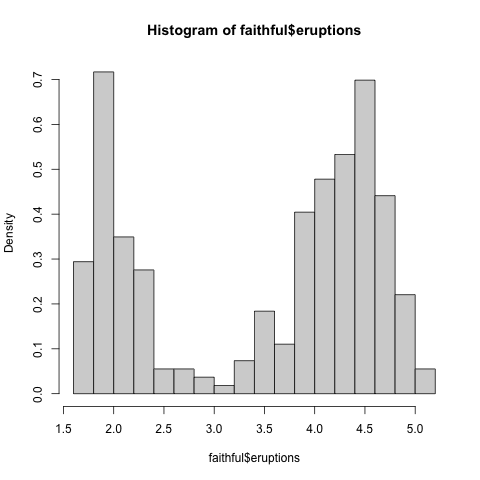
\includegraphics[width=3.0in]{FaithfulDuration.png}
}
\caption{Old Faithful eruption durations}
\label{faithfulhist}
\end{figure}

\begin{figure}[tb]
\centerline{
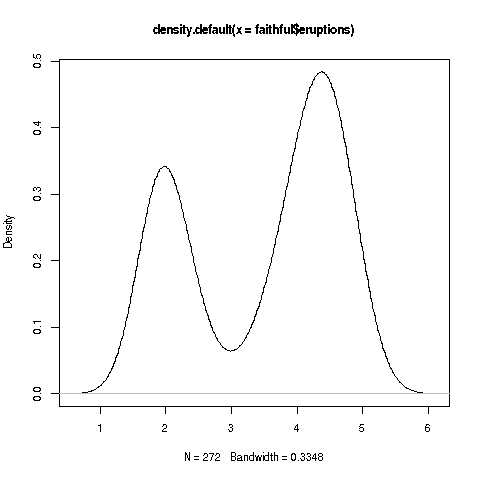
\includegraphics[width=3.0in]{FaithfulDurationSmooth.png}
}
\caption{Old Faithful eruption times, smoothed}
\label{faithfulhistsmooth}
\end{figure}

Assuming there really are two types of eruptions, our hidden state $S_j$
for the $j^{th}$ eruption in our dataset is the type of eruption.  $Y_j$
is the duration of that eruption.  Again, the $S_j$ are unobserved.

Our objective is to use the $Y_j$ data to estimate $\pi$, the proportion
of type 1 eruptions, and
$
\mu_1,
\mu_2,
\sigma_1 
\textrm{ and }
\sigma_2 
$, the means and standard deviations of the assumed normal distributions
for duration in the two eruption types.

% \subsection{``Hidden'' States}
% 
% In the network example, the hidden state is whether we are currently in
% a clear period (coded 1) or a noisy period (coded 2).  The observed
% state is the actual received bit.
% 
% For the purposes of the discussion here, let's take as our geyser model
% that of O'Hara \textit{et al} cited above.  Our \textit{hidden}, i.e.\
% unknown, state here will be the identity of the currently eruption type,
% long (coded 1) or short (coded 2) Our \textit{observed} state is the
% duration of the eruption.  Note the overlap: some durations
% for type 1 eruptions may actually be shorter than some durations
% for eruptions of type 2.

\subsection{Number of States}

In many applications, a major part of the modeling process is deciding
on the number of states.  In our models above, it is natural to take
this number to be 2, but generally there is no obvious such number.  In
such cases, we have a classic model-fitting choice, a famous principle
in model fitting:

\begin{quote}

The \textit{Bias-Variance Tradeoff}.  

Say we wish to predict human weight from height.  We wish to estimate
the function $w(t) = E(W | H = t)$, the relation between weight and
height in our population.  We might try a linear model for $w(t)$, but a
quadratic model would give use greater flexibility.  A cubic model be
even more general, and so on.

From the notion of a Taylor series in calculus\footnote{Or for those
with a background in real analysis, the Stone-Weierstrass Theorem.},
one might think that the higher the degree of the fitted polynomial, the
better.  But that is merely saying that higher-degree models have
smaller model bias, and counteracting that is the problem of sampling
error.  The higher the degree, the more the sampling error (called the
\textit{standard error} in statistics).  So, we need larger datasets
for higher-degree models.

If we are on the ``wrong'' side of this tradeoff, the model is said to
be \textit{overfit}.

\end{quote}

So, the more hidden states in our model, the smaller the model bias but
the larger the ampling error; setting the number of hidden states at too
large a level will result in overfitting.

For instance, consider financial time series data, such as daily stock
market data.  The \textbf{sp500} dataset, included with some software we
will use below, consists of 772 days of the Standard and Poor market
average.  In the book associated with the software,\footnote{\textit{Mixture and
Hidden Markov Models with R,} by Ingmar Visser and Maarten
Speekenbrink, Springer.} the authors postulate 2 hidden states, ``bull''
and ``bear'' sentiments among the traders, and fit an HMM accordingly.
With 3 states, 4 states and so on, we might achieve more accuracy, 
but eventually the Bias-Variance Tradeoff will result in overfitting.

Simiarly, the \textbf{faithful} dataset consists of only 272
observations, for instance.  And though the choice of 2 states in that
example does not seem large relative to 272, we will see below that we
are maximizing a certain quantity over an enormous number of choices,
again raising the possibility of overfitting.

\subsection{Time (and ``Time'')}

In spite of sharing the property of having hidden states, and the $Y|S$
structure, there is a fundamental difference between the battery example
above and the other two.  In the battery case, the pairs $(S_j,Y_j)$ are
iid, while in the network and geyser examples they are sequential in
time; there is a time dependency between each pair and the next.  The
stock market example is also sequential.

In some cases ``time'' may correspond to postion, say in HMM genomics
models, but again, the sequential nature is key.  That is what
distinguishes HMMs from MMs.

\subsection{Conditional Probabilities of Observed Values}

Let $S$ denote the hidden state, and let $Y$ denote the corresponding
observed value.  A major ingredient in the analysis will be expressions of
the form

\begin{equation}
P(Y = w | S  = v)
\end{equation}

If $Y$ is continuous rather than discrete, the above expression would be
something like

\begin{equation}
f_{Y|S} (w,v) 
\end{equation}

where $f_{Y|S}$ is the conditional density of $Y$ given $S$:

\begin{equation}
f_{Y|S}(w,v) 
= \frac{d}{dw} F_{Y|S}(w,v) 
= \frac{d}{dw} P(Y \leq w ~|~ S = v)
\end{equation}

These conditional distribution quantities are then used to estimate
model parameters, as we will see below.\footnote{The word
\textit{estimate} is vital here.  As with any statistical method, our
results are just estimates of population values, and the larger our
sample, the more likely our estimate is to the true value.}

% \subsection{Mixture Models vs.\ HMMs: the 10,000 Foot View}
% 
% Both types of models have hidden and observed states.  But HMMs add an
% extra aspect:  We model the system as evolving in time, with
% probabilities of going from one state to another at each time step.  So
% this is a dynamic model, while MMs are static. 
% 
% In the Old Faithful example, for instance, in an MM we may wish to
% estimate the overall proportion of eruptions of type 1, while in an
% HMM we may wish to have an estimated probability that the \textit{next}
% eruption is of that type.
% 
% Another example is a financial dataset included in the HMM software we will
% use.  The (hypothetical) hidden state is whether the stock market
% sentiment is in a ``bull'' or ``bear'' mood.  The market, of course,
% definitely has a time component, daily, hence the HMM analysis.  But the
% authors also do a static analysis, looking at the data as a whole in a
% way similar to the static geyser analysis.

\section{Mixture Models}

Actually, MMs are typically not presented in the conditional distribution
form we saw above.  Let's see how to reconcile the standard description
with what we saw above.

\subsection{Definition}
\label{mixdef}

Say $Y$ is discrete.  Then

\begin{equation}
P(Y = w) = \sum_{v} P(S = v) ~ P(Y = w | S = v)
\end{equation}

So in terms of cumulative distribution functions (cdfs),

\begin{equation}
\label{mixedFs}
F_Y(w) = P(Y \leq w) = 
\sum_{v} P(Y \leq w | S = v) ~ P(S = v) =
\sum_{v} c_v F_{Y|S}(w,v)
\end{equation}

where 

\begin{equation}
c_v = P(S = v)
\end{equation}

Speaking just in terms of cdfs, we say that $F_Y$ is a \textit{mixture}
of the cdfs $F_{Y|S}$, which simply means that $F_Y$ is a linear
combination of the $F_{Y|S}$, where the coefficients are nonnegative
numbers whose sum is 1.\footnote{In math parlance, we say that $F_Y$ is
a \textit{convex} combination of the $F_{(Y|S)}$..}

Now consider random variables $X_1,...,X_k$, with cdfs $F_{X_i}$ (not
necessarily independent),\footnote{I use ``X'' for my variable name
rather than ``Y,'' to emphasize the mainly implicit nature of states.}
and let $d_i, ~ i=1,...,k$ be nonnegative
numbers whose sum is 1.  Define the random variable $W$ to take on the
value $X_i$ with probability $d_i$, $i=1,...,k$.  Then we say that $W$
has a mixture distribution.  With this view, the state is only implicit.

Note that

\begin{equation}
F_{W}(t) = \sum_{i=1}^k d_i F_{X_i}(t)
\end{equation}

Similar relations hold for probability mass functions ($X_i$ discrete)
and density functions ($X_i$ continuous).

In MM analysis, the usual quantities of interest are the 
$F_{X_i}$ and the $d_i$.  In the Old Faithful example, the former 
typically means using the data to somehow estimate the means and
standard deviations of the two normal distributions, and the proportions
of eruptions of the two types.

\subsection{Cluster Analysis}

The $X_i$ can be vector-valued, and this is the basis for
\textit{cluster analysis}, a major field in machine learning/data
science.

\subsection{The EM Algorithm}

Probably the most common approach to estimating such quantities is the
\textit{EM algorithm}.  We will present the details in Section
\ref{emalg}, but will make use of it now, so let's at least look at an
overview here.

Say the distribution of some probabilistic quantity, depends on two sets
of parameters, say $\theta$ and $\gamma$.  The algorithm works like
this:  We set initial guesses, $\theta_0$ and $\gamma_0$ for the two
parameter sets, then update alternately, first finding a new guess for
$\theta$ based on our latest guess for $\gamma$, then vice versa.  Of
course, we also make use of our dataset at every step.

In the geyser example, $\theta$ is consists of the two means and two
standard deviations, of the two normal distributions.  $\gamma$ is the
proportions of the two normal distributions, i.e.\ the $c_v$ in Equation
(\ref{mixedFs}).

\begin{enumerate}

\item Set initial guesses, $\theta_0$ and $\gamma_0$.

\item Form a new guess for $\theta$, denoted $\theta_1$, based
on $\gamma_0$.

\item Form a new guess for $\gamma$, denoted $\gamma_i$, based
on $\theta_i$.

\end{enumerate} 

LATER, IN THE HMM SECTION, WE HAVE THETA AS THE MARKOV MATRIX, AND GAMMA
AS THE MLE STATE SEQUENCE.

\subsection{The mixtools Package}

This is a large package with many functions for analysis of MMs.  The EM
algorithm is used extensively.  Here we will illustate the function
\textbf{normalmixEM()}, which as the name implies, fits an MM of normal
distributions.  Again, for the sake of simplicity, we will cover only a
few of the many features of this function.

The algorithm is iterative, and thus requires initial guesses for the
means/standard deviations of the two normal distributions, and the
proportions of the two eruption types.  I took the former (arguments
\textbf{mu} and \textbf{sigma}) from the appearance of the histogram,
and used equal weights for the latter (argument \textbf{lambda}.

\begin{lstlisting}
> mixout <- normalmixEM(faithful$eruptions,
   lambda=0.5,mu=c(55,80),sigma=10,k=2) number of iterations= 9 
> str(mixout)
List of 9
 $ x         : num [1:272] 79 54 74 62 85 55 88 85 51 85 ...
 $ lambda    : num [1:2] 0.361 0.639
 $ mu        : num [1:2] 54.6 80.1
 $ sigma     : num [1:2] 5.87 5.87
 ...
\end{lstlisting}

So, the estimate from EM is that about 36\% of the eruptions are of type
1.  The estimated mean eruption durations for the two eruption types
are 54.6 and 80.1.

\subsection{Vector-Valued X}

The most common mixture modeling is in \textit{cluster analysis}, often
referred to as \textit{unsupervised learning}.  We have multivariate
data, say in a marketing application, and wish to find meaningful
subgroups, say different types of customers.  Again, we don't know what
types are there, if there are any in some sense, but if we can find
some, this may be very useful.

The \textbf{faithful} data is bivariate, with columns for both eruption
duration and waiting time between eruptions.  A plot, seen in Figure
\ref{bivariatefaithful}, does seem to show two groups.  Of course, if
there really are two groups, we can't tell for sure here which point
belongs to which group, but again, in say, a marketing context, we just
want to identify rough groups.  

\begin{figure}[tb]
\centerline{
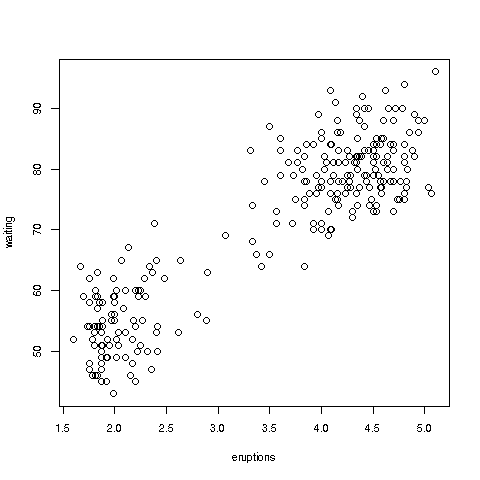
\includegraphics[width=3.0in]{BivarFaithful.png}
}
\caption{Old Faithful bivariate plot}
\label{bivariatefaithful}
\end{figure}

In the univariate case, we assumed normal distributions for the
components.  The \textbf{mixtools} function \textbf{mvnormalmixEM()} 
fits a multivariate normal model.  I tried running it completely on the
basis of the argument defaults:

\begin{lstlisting}
> mvnout <- mvnormalmixEM(fMaithful)
number of iterations= 12 
> str(mvnout)
List of 9
 $ x         : num [1:272, 1:2] 3.6 1.8 3.33 2.28 4.53 ...
  ..- attr(*, "dimnames")=List of 2
  .. ..$ : chr [1:272] "1" "2" "3" "4" ...
  .. ..$ : chr [1:2] "eruptions" "waiting"
 $ lambda    : num [1:2] 0.356 0.644
 $ mu        :List of 2
  ..$ : num [1:2] 2.04 54.48
  ..$ : num [1:2] 4.29 79.97
 $ sigma     :List of 2
  ..$ : num [1:2, 1:2] 0.0692 0.4352 0.4352 33.6973
  ..$ : num [1:2, 1:2] 0.17 0.941 0.941 36.046
...
\end{lstlisting}

Since our data is bivariate, the estimated mean for each cluster has
is a vector of length 2, with a 2 $\times$ 2 covariance matrix.  The
estimates are displayed in the above output.  The \textbf{lambda} output
again shows the estimated mixing proportions, similar to the ones we
found in the univariate case.

Cluster analysis is a vast topic.  Estimation via the EM algorithm is
only one of many methods to choose from.

\subsection{Mean and Variance of Random Variables Having Mixture
Distributions}
\label{mixmeanvar}

Think of the random variables S and Y in Section \ref{mixdef}.
Then EY follows the Law of Total Expectation:

\begin{equation}
\label{mixmean}
EY = E[E(Y | S)]
\end{equation}

Of course, evaluating this would require being able to compute E(Y $|$
S), which is easy in some cases, not so easy in others.

Also, using the Law of Total Variance, we have that

\begin{equation}
\label{mixvar}
Var(Y) = E[Var(Y|S)] + Var[E(Y|S)]
\end{equation}

\section{Hidden Markov Models}

As noted, we have an observable variable $Y$, and a state $S$, but now
the state evolves in time, resulting in our data
$
(S_1,Y_1),
(S_2,Y_2),
...,
(S_n,Y_n),
$

The time pattern is assumed to be \textit{Markovian}, or ``memoryless'':

\begin{equation}
P(S_{k+1} = v_{k+1} ~|~ S_1 = v_1, S_2 = v_2, ...  S_k = v_k) =
P(S_{k+1} = v_{k+1} ~|~ S_k = v_k) 
\end{equation}

In English,

\begin{quote}
The probability of a future event, given the present and the past,
depends only on the present.
\end{quote}

The states $S_i$ are unobserved, i.e.\ ``hidden,'' but note that also it
may be real, as in our noisy network example, or just postulated, as in
the geyser example.  In an analysis of the stock market, for instance,
one might postulate ``bull'' and ``bear'' moods among the traders.

\begin{lstlisting}

> z <- hmmr::hmm(faithful$eruptions,2)
> summary(z)
Initial state probabilities model 
pr1 pr2 
  1   0 

Transition matrix 
        toS1  toS2
fromS1 0.479 0.521
fromS2 0.938 0.062

Response parameters 
Resp 1 : gaussian 
    Re1.(Intercept) Re1.sd
St1           4.289  0.413
St2           2.036  0.263

# z is an S4 class, one of whose components, posterior, is a data frame
> z@posterior$state
  [1] 1 2 1 2 1 2 1 1 2 1 2 1 1 2 1 2 2 1 2 1 2 2 1 1 1 1 2 1 1 1 1 1 1 1 1 2 2
 [38] 1 2 1 1 2 1 2 1 1 1 2 1 2 1 1 2 1 2 1 1 2 1 1 2 1 2 1 2 1 1 1 2 1 1 2 1 1
 [75] 2 1 2 1 1 1 1 1 1 2 1 1 1 1 2 1 2 1 2 1 2 1 1 1 2 1 2 1 2 1 1 2 1 2 1 1 1
[112] 2 1 1 2 1 2 1 2 1 2 1 1 2 1 1 2 1 2 1 2 1 2 1 2 1 2 1 2 1 1 2 1 1 1 2 1 2
[149] 1 2 1 1 2 1 1 1 1 1 2 1 2 1 2 1 1 1 2 1 2 1 2 2 1 1 1 1 1 2 1 1 2 1 1 1 2
[186] 1 1 2 1 2 1 2 1 1 1 1 1 1 2 1 2 1 1 2 1 2 1 1 2 1 2 1 2 1 1 1 2 1 2 1 2 1
[223] 2 1 1 1 1 1 1 1 1 2 1 2 1 2 2 1 1 2 1 2 1 2 1 1 2 1 2 1 2 1 1 1 1 1 1 1 2
[260] 1 1 1 2 1 2 2 1 1 2 1 2 1

\end{lstlisting}

\section{The EM Algorithm} 
\label{emalg}

Now returning to our main topic of mixture models, let's discuss a very
common tool for fitting such models.

Consider again the example in Section \ref{oldtrick}.  Now suppose p, q
and r are all unknown, and we wish to estimate them from data. Say we
will perform the above experiment 50 times, resulting in our data
$N_1,...,N_{50}$ We will estimate p, q and r by applying some method,
say the Method of Moments, Maximum Likelihood or some ad hoc method of
our own, to our data. Each $N_i$ has the distribution seen in $p_N$
above. This is a parametric family, with 3 parameters. (If, say, r is
known, we only have a two-parameter family, and things are easier.)

So, how can we estimate those three parameters?  In Chapter
\ref{chap:est}, we found some general methods for parameter estimation.
Let's look at one of them, Maximum Likelihood Estimators (MLEs).

In (\ref{mixbinom}), the MLE vector 
$(\widehat{p},
  \widehat{q},
  \widehat{r})'$
would be found by maximizing

\begin{equation}
\Pi_{i=1}^n
\left [ r \binom{10}{N_i} p^{N_i} (1-p)^{10-N_i} +
(1-r) \binom{10}{N_i} q^{N_i} (1-q)^{10-N_i}
\right ]
\end{equation}

After taking derivatives, etc., one would end up with a messy, nonlinear
set of equations to solve.  One could try {\bf mle()}, but there is a
better way to get the MLE: the Expection/Maximization (EM) algorithm.
The derivation and ultimate formulas can get quite complex.
Fortunately, R libraries exist, such as {\bf mixtools}, so you can avoid
knowing all the details, as long as you understand the basic notion of a
mixture model.  

In something like (\ref{hsum}), for instance, one would make initial
guesses for the $p_M(i)$ and then estimate the parameters of the $g_i$.
In the next step, we'd do the opposite---take our current guesses for
the latter parameters as known, and estimate the $p_M(i)$.  Keep going
until convergence.

To make things concrete, recall the trick coin example Section
\ref{oldtrick}.  But change it a little, so that the probabilities of
heads for the two coins are unknown; call them $p_0$ (heads-light coin)
and $p_1$ (heads-heavy coin).  And also suppose that the two coins are
not equally likely to be chosen, so that $p_M()$ is not known; denote
P(M = 1) by q.

Suppose we have sample data, consisting of doing this experiment
multiple times, say by reaching into the box n times and then doing m
flips each time.  We then wish to estimate 3 quantities---q and the two
$p_i$---using our sample data.  

We do so using the following iterative process.  (The account here is
not exactly EM, but captures the spirit of it.) We set up initial
guesses, and iterate until convergence:

\begin{itemize}

\item {\bf E step:} Update guess for q (complicated Bayes Rule equations).

\item {\bf M step:} Using the new guess for q, update the gueses for the
two $p_i$.

\end{itemize}

The details are beyond the scope of this book.\footnote{``M'' in the M
step refers to the Maximum Likelihood method, a special case of the
material in Section \ref{mle}.}

\subsection{Example:  Two Kinds of Batteries}

Say a factory produces two kinds of batteries.  One kind has lifetime
that is exponentially distributed with mean 200 and the other's
distribution is exponential with mean 500.  Suppose 60\% of the
factory's production is of the former type, with 40\% being of the
latter type.  Let's find the mean and variance of the lifetime Y of a
randomly chosen battery.

Note that the distribution of Y is a mixture, in the sense of Section
\ref{genmix}, in particular (\ref{continmix}).  Y here is a continuous
random variable, referred to in that section as the ``continuous
outcome'' case.   In the notation there, let M be the battery type, with
M being 0 or 1, for the 200-hour and 500-hour batteries, respectively.
The conditional density of Y given M = 0 is exponential with mean 200,
while given M = 1 it is exponential with mean 500.  The unconditional
density of Y is the mixture of these two exponential densities, as 
(\ref{continmix}).

We want to find the \underline{un}conditional mean and variance of Y.

Then

\begin{equation}
\label{batt1}
E(Y|M)=\left\{ \begin{array}{rl}
200, & w.p. ~ 0.60 \\
500, & w.p. ~ 0.40
\end{array}\right. 
\end{equation}

and 

\begin{equation}
\label{batt2}
Var(Y|M)=\left\{ \begin{array}{rl}
200^2, & w.p. ~ 0.60 \\
500^2, & w.p. ~ 0.40
\end{array}\right. 
\end{equation}

(recalling that in the exponential family, variance is the square of the
mean).

We can now use the formulas in Section \ref{mixmeanvar}.  Let $Q_1 =
E(Y|M)$  and $Q_2 = Var(Y|M)$.  Then

\begin{equation}
EY = EQ_1 = 0.60 \times 200 + 0.40 \times 500
\end{equation}

and 

\begin{eqnarray}
Var(Y) &=& E(Q_2) + Var(Q_1) \\
&=& (0.60 \times 200^2 + 0.40 \times 500^2) + Var(Q_1) \\
&=& (0.60 \times 200^2 + 0.40 \times 500^2) + E(Q_1^2) - (EQ_1)^2 \\
&=& (0.60 \times 200^2 + 0.40 \times 500^2) + (0.60 \times 200^2 + 0.40
\times 500^2)  \\
& & - (0.60 \times 200 + 0.40 \times 500)^2 \\
\end{eqnarray}

\subsection{Example:  Overdispersion Models}

A common model used in practice is that of {\bf overdispersion}, in
connection with Poisson models.  

Recall the following about the Poisson distribution family:

\begin{itemize}

\item [(a)] This family is often used to model counts.

\item [(b)] For any Poisson distribution, the variance equals the mean.

\end{itemize}

In some cases in which we are modeling count data, condition (b) is too
constraining.  We want a ``Poisson-ish''
distribution in which the variance is greater
than the mean, called {\bf overdispersion}.  

One may then try to fit a mixture of several Poisson distributions,
instead of a single one.  This does induce overdispersion, as we will
now see.  

Suppose M can equal 1,2,...,k, with probabilities $p_1,...,p_k$ that sum
to 1.  Say the distribution of Y given M = i is Poisson with parameter
$\lambda_i$.  Then Y has a mixture distribution.  Our goal here will be
to show that Y is overdispersed, i.e. has a large variance than mean.

By the Law of Total Expectation,

\begin{eqnarray}
\label{meanlamb}
EY &=& E[E(Y|M)] \\ 
&=& E(\lambda_M) \label{elambm} \\
&=& \sum_{i=1}^k p_i \lambda_i
\end{eqnarray}

Note that in the above, the expression $\lambda_M$ is a random variable,
since its subscript M is random.  Indeed, it is a function of M, so
Equation (\ref{egofx}) then applies, yielding the final equation.  The
random variable $\lambda_M$ takes on the values $\lambda_1,...,\lambda_k$
with probabilities $p_1,...,p_k$, hence that final sum.

The corresponding formula for variance, (\ref{bis}), can be used to
derive Var(Y).

\begin{eqnarray}
Var(Y) &=& E[Var(Y|M)] + Var[E(Y|M)] \\ 
&=& E(\lambda_M) + Var(\lambda_M) \label{thislast} \\
&=& EY + Var(\lambda_M) \label{thislast} \\
\end{eqnarray}

Did you notice that this last equation achieves our goal of showing
overdispersed?  Since

\begin{equation}
Var(\lambda_M) > 0
\end{equation}

we have that

\begin{equation}
Var(Y) > E(\lambda_M) = EY
\end{equation}

by (\ref{elambm}).

But let's see just how much greater the variance is than the mean.  The
second term in (\ref{thislast}) is evaluated the same way as in
(\ref{elambm}):  This is the variance of a random variable that takes on
the values $\lambda_1,...,\lambda_k$ with probabilities $p_1,...,p_k$,
which is

\begin{equation}
\sum_{i=1}^k p_i (\lambda_i - \overline{\lambda})^2
\end{equation}

where 

\begin{equation}
\overline{\lambda} =  E\lambda_M = \sum_{i=1}^k p_i \lambda_i
\end{equation}

Thus

\begin{equation}
EY = \overline{\lambda}
\end{equation}

and

\begin{equation}
Var(Y) = \overline{\lambda} + 
\sum_{i=1}^k p_i (\lambda_i - \overline{\lambda})^2
\end{equation}

So, as long as the $\lambda_i$ are not equal, we have

\begin{equation}
Var(Y) > EY
\end{equation}

in this Poisson mixture model, in contrast to the single-Poisson case
in which Var(Y) = EY.  You can now see why the Poisson mixture model is
called an overdispersion model.

So, if one has count data in which the variance is greater than the
mean, one might try using this model.

In mixing the Poissons, there is no need to restrict to discrete M.  In
fact, it is not hard to derive the fact that if X has a gamma
distribution with parameters r and p/(1-p) for some $0 < p < 1$, and Y
given X has a Poisson distribution with mean X, then the resulting Y
neatly turns out to have a negative binomial distribution.

% Again, there may be a computability issue.  But see the examples below.

% \section{Example:  Cluster Analysis}
% 
% We will in Section \ref{mixclust} see that the notion of mixtures can
% also be applied to clustering.
% 
% \section{Markov Chain with Random $X_0$}
% 
% LOSE MARKOV PROPERTY
% 
% \section{Bayes Models, Including Empiricial Bayes}
% 
% JUST REFER TO THE BAYES SECTION, BUT NOTE IN THE LATTER THAT IT IS A
% MIXTURE

% \section{De Finetti's Theorem}
% 
% Consider again the trick coin example, Section \ref{oldtrick}.  As we
% have discussed, the tosses $B_i$ are not independent.  However, they are
% {\bf exchangeable}:
% 
% \begin{equation}
% P(B_
% \end{equation}


\end{document}

> x <- geyserSim(100000,0.9,0.3)
> z <- hmmr::hmm(x,2)
> summary(z)
Initial state probabilities model
pr1 pr2
  1   0

Transition matrix
        toS1  toS2
fromS1 0.681 0.319
fromS2 0.891 0.109

Response parameters
Resp 1 : gaussian
    Re1.(Intercept) Re1.sd
St1          -0.016  0.991
St2           1.959  1.018

geyserSim <- function(nTimePers,AtoB,BtoA)
{
   x <- vector(length=nTimePers)
   state <- 'A'
   for (i in 1:nTimePers) {  # could use rgeom() and while{} instead
      # check for state change
      if (state == 'A') {
         if (runif(1) < AtoB)  # now bad network
            state <- 'B'
      } else {  # state == 'B'
         if (runif(1) < BtoA)  # now bad network
            state <- 'A'
      }
      if (state == 'B') x[i] <- rnorm(1)
      else x[i] <- rnorm(1) + 2
   }
   x
}

netSim <- function(nBits,goodToBadProb,badToGoodProb,badProb0) 
{
   trueBits <- sample(0:1,nBits,replace=TRUE)
   rcvdBits <- trueBits  
   state <- 'good'
   for (i in 1:nBits) {  # could use rgeom() and while{} instead
      # check for state change 
      if (state == 'good') {
         if (runif(1) < goodToBadProb)  # now bad network
            state <- 'bad'
      } else {  # state == 'bad'
         if (runif(1) < badToGoodProb)  # now bad network
            state <- 'good'
      }
      if (state == 'bad' && runif(1) < badProb0)
         rcvdBits[i] <- 0
   }
   cbind(trueBits,rcvdBits)
}



